\documentclass[12pt,handout]{beamer}

%\documentclass{beamer}
\usetheme{Boadilla}
\useoutertheme{split}
\usepackage{fancyvrb}
\usepackage{tikz}
\usepackage{svg}
\usetikzlibrary{shapes, calc, shapes, arrows, datavisualization}

\usepackage{amsmath,amssymb}

\definecolor{myblue}{RGB}{80,80,160}
\definecolor{exerciseblue}{RGB}{200, 200, 247}
\definecolor{mygreen}{RGB}{80,160,80}


\title{Linear Programming Algrebra}
\author{Abr\'emod Training}
\titlegraphic{
\includegraphics[scale=0.1]{abremodlogo.png}}


\begin{document}

\begin{frame}
\titlepage
\end{frame}

\begin{frame}
\frametitle{Overview}
\begin{itemize}
\item Linear Programming Geometry
\item Linear Programming Algebra
\item Duality
\item Sensitivity Analysis
\begin{itemize}
\item Dual Values
\item Reduced Costs
\end{itemize}
\end{itemize}
\end{frame}

\begin{frame}
\frametitle{Linear Programming Geometry}
\vskip -0.05 in
\tiny
\begin{eqnarray}
\max_{x,y} && z = 6x + 4y \nonumber \\
\mbox{s.t.} && x + y \le 6 \\
&& 2x + y \le 9 \\
&& 2x + 3y \le 16 \\
&& x, y \ge 0 \nonumber
\end{eqnarray}
\vskip -0.07 in
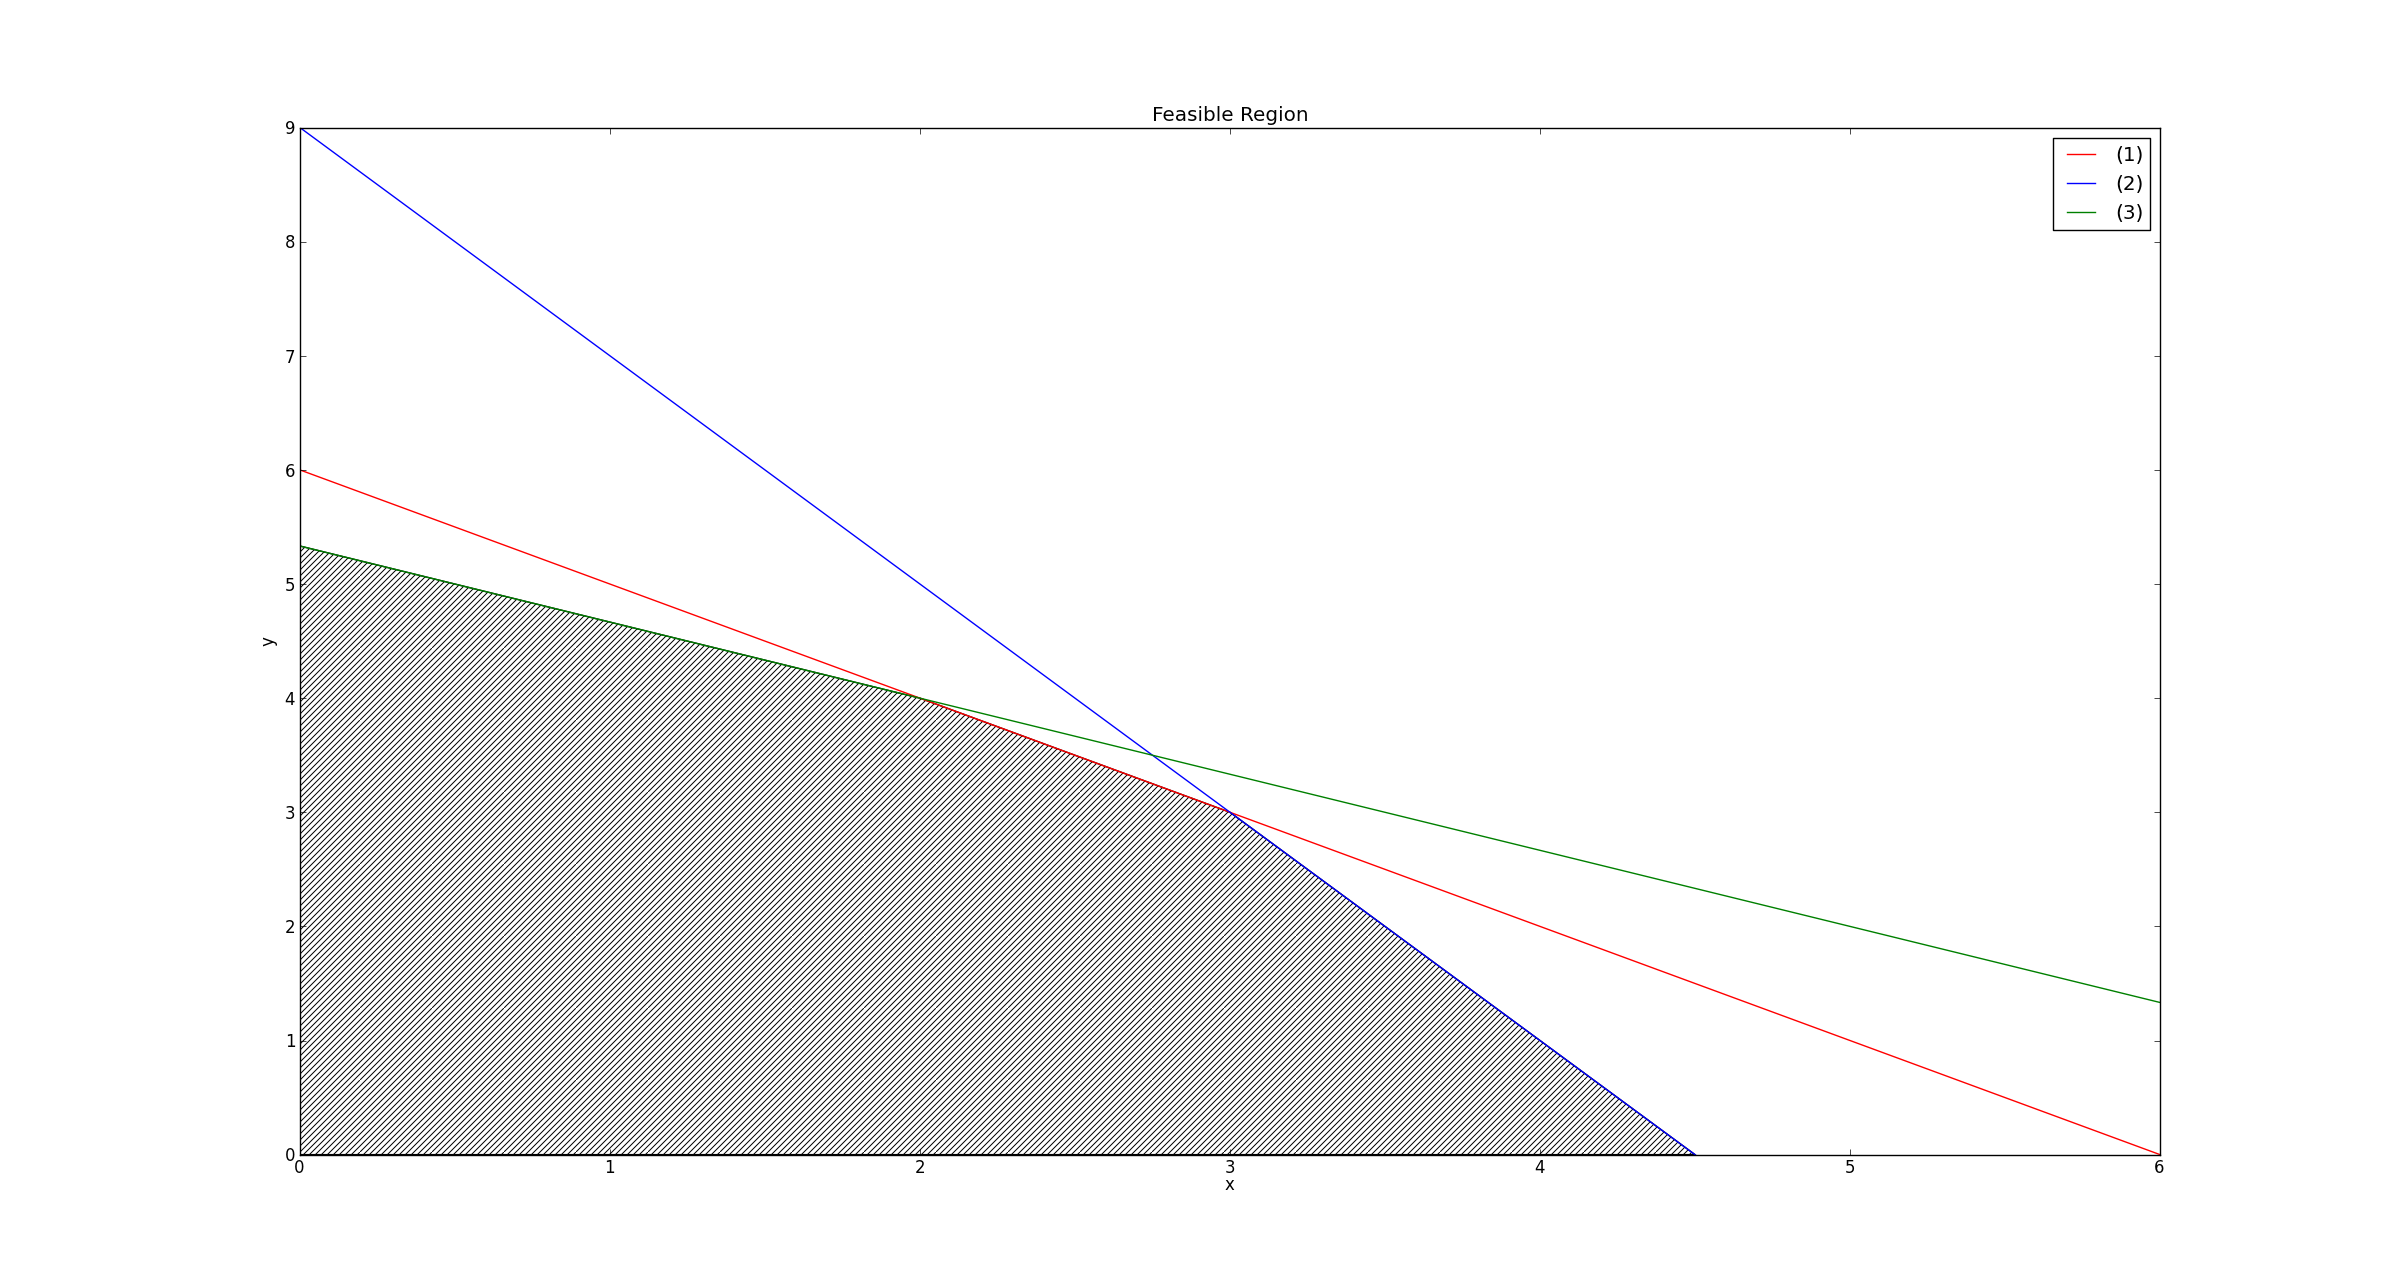
\includegraphics[scale=0.2]{feasible_region.png}
\end{frame}

\begin{frame}
\frametitle{Linear Programming Geometry}
\scriptsize
\begin{itemize}
\item Plot the objective function $z = 6x + 4y$ for some fixed values of $z$.
\item These are the so-called {\em isoprofit lines} or {\em objective function contours}.
\item Increasing $z$ results in a parallel shift to the right.
\end{itemize}
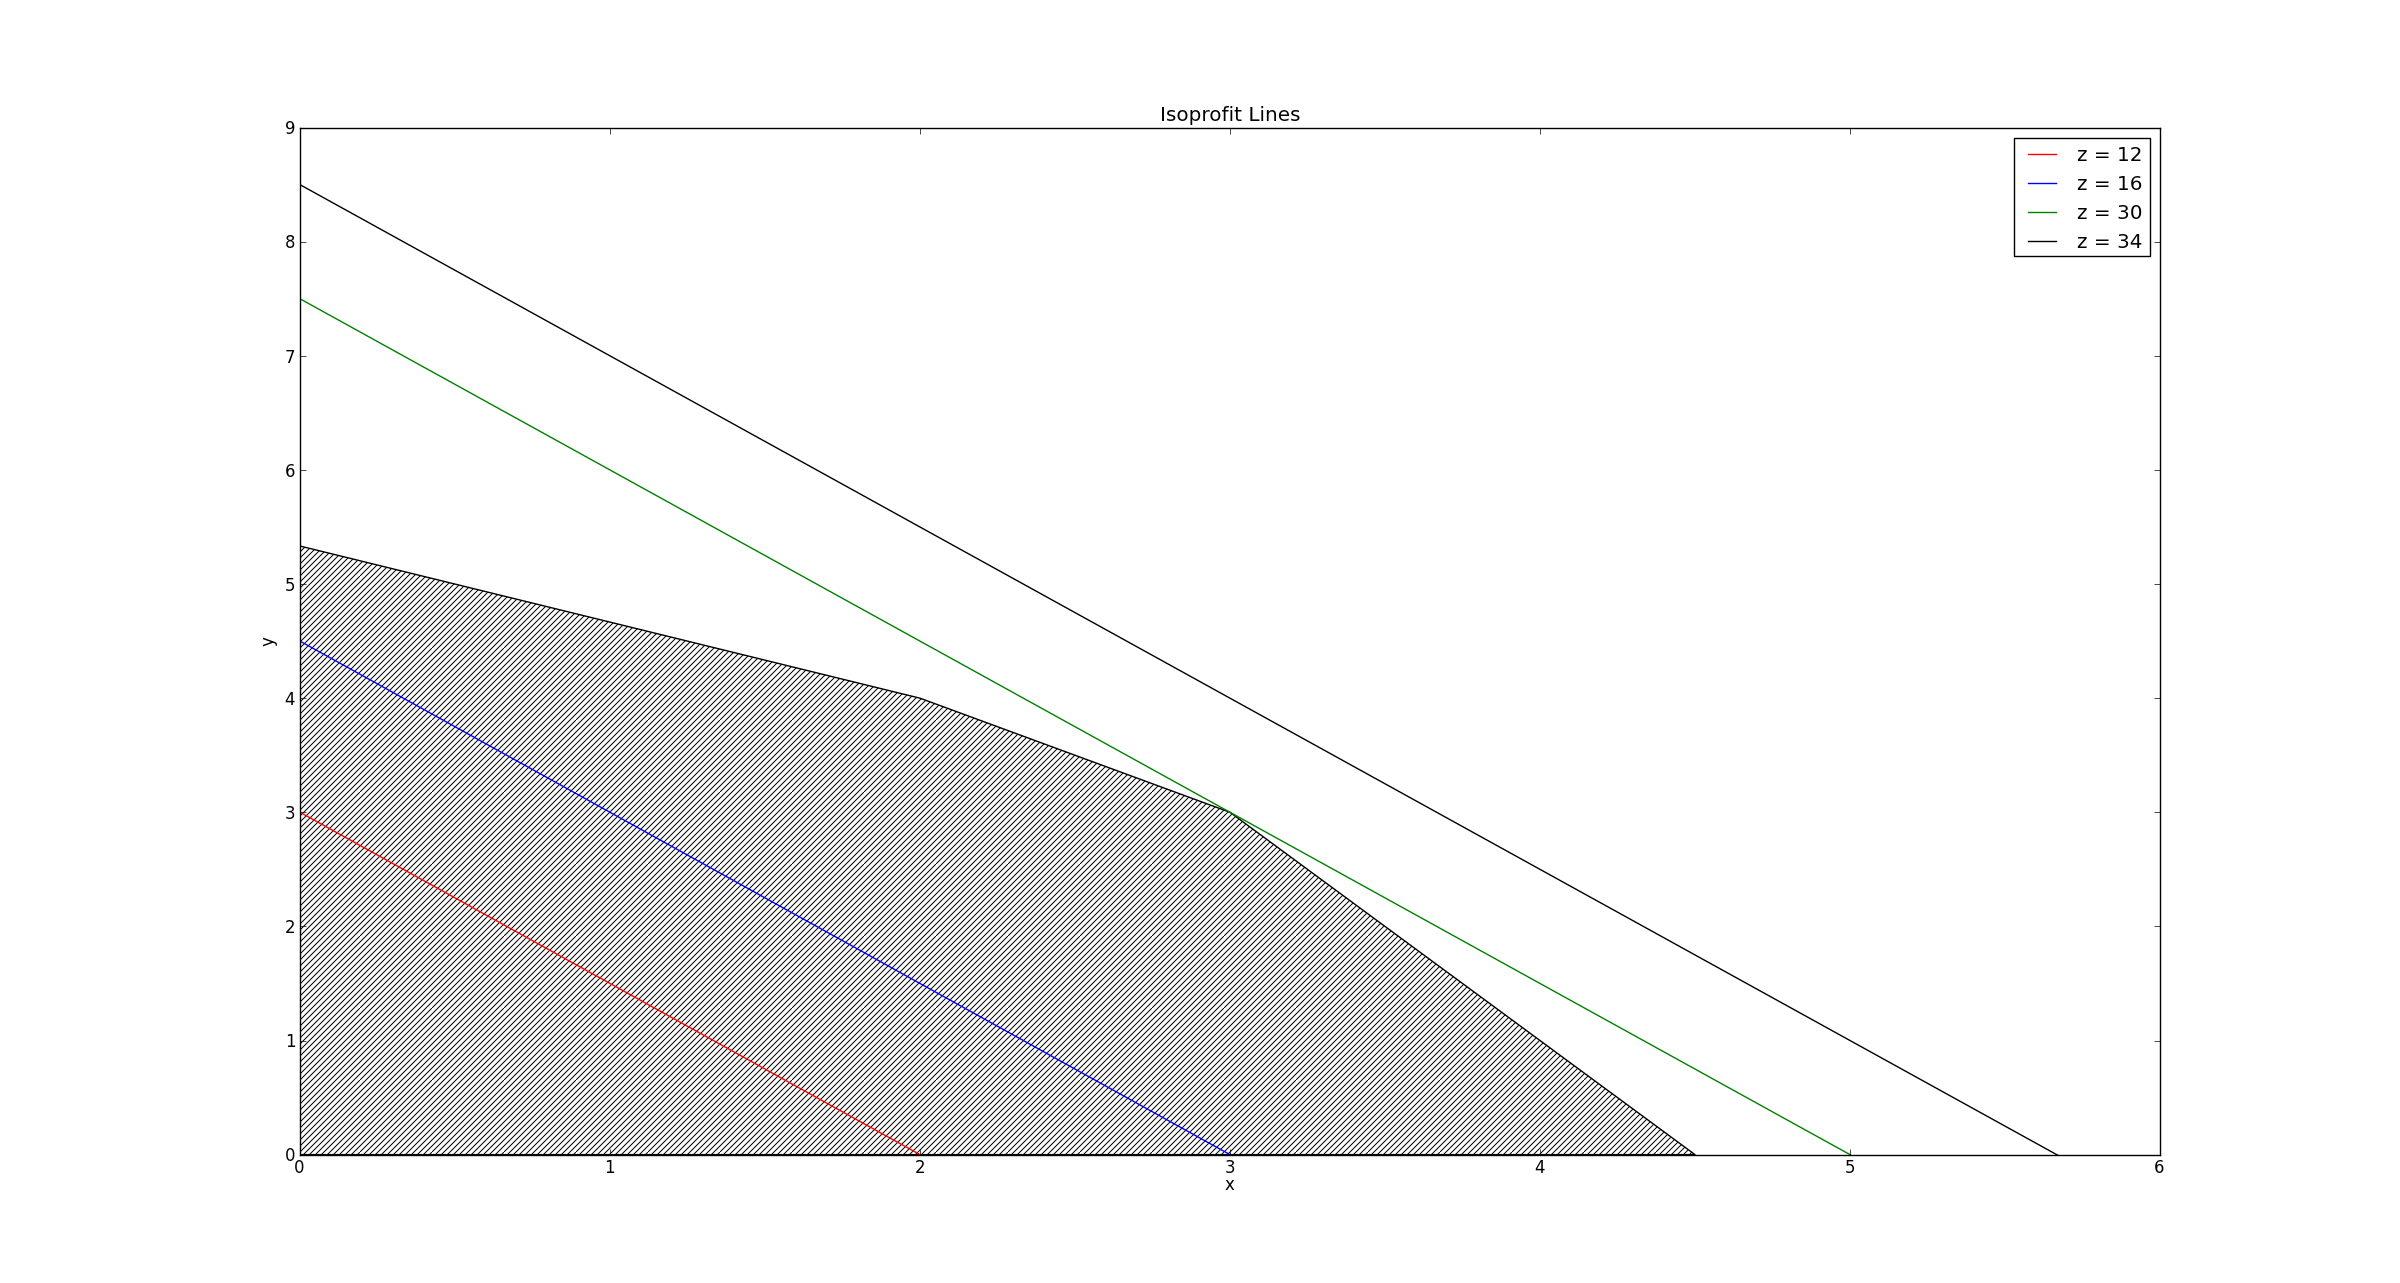
\includegraphics[scale=0.2]{isoprofit_lines.png}
\end{frame}

\begin{frame}
\frametitle{Observations}
\begin{itemize}
\item Feasible region of a linear program is always a convex polyhedron
\item At least one optimal solution occurs at a corner point (a.k.a. extreme point or vertex) of this polyhedron
\item Infinitely-many points in the feasible region, but only finitely many corner points
\end{itemize}
\end{frame}


\begin{frame}
\frametitle{Linear Programming Algebra}
First, how to solve linear systems of equations?
\begin{eqnarray}
2 x_1 + 1 x_2 + 1 x_3 &=& 4 \nonumber \\
4 x_1 - 6 x_2 + 0 x_3 &=& 2 \nonumber \\
-2 x_1 + 7 x_2 + 2 x_3 &=& 1 \nonumber
\end{eqnarray}
Systematically perform row operations to form equivalent systems
\begin{center}
Row 1 $\leftarrow \frac{1}{2}$ Row 1 \\
Row 2 $\leftarrow$ Row 2 - 4 Row 1 \\
Row 3 $\leftarrow$ Row 3 + 2 Row 1 \\
$\vdots$ \\
\end{center}
Until we arrive at an equivalent system with an obvious solution
\begin{eqnarray}
1 x_1 + 0 x_2 + 0 x_3 &=& 2 \nonumber \\
0 x_1 + 1 x_2 + 0 x_3 &=& 1 \nonumber \\
0 x_1 + 0 x_2 + 1 x_3 &=& -1 \nonumber
\end{eqnarray}
\end{frame}

\begin{frame}
\frametitle{Linear Programming Algebra}
\begin{itemize}
\item These row operations correspond to multiplying equations by constants and adding the result to other equations.
\item ``Systematically'' performing row operations means picking an equation and solving for a specific variable, then eliminating that variable in all other equations.
\item For a square system that has an equal number of variables and equations, it is relatively easy to decide which equation to solve and which variable to solve for.
\item If the system has a unique solution, we can solve for the $i$th variable in the $i$th equation, swapping the order of equations as needed.
\end{itemize}
\end{frame}

\begin{frame}
\frametitle{Linear Programming Algebra}
Linear programs typically have:
	\begin{itemize}
	\item More variables than equations.
	\item More than one feasible solution (almost always).
	\item More than one optimal solution (more often than you might think).
	\end{itemize}
This being said, we can still solve LPs via systematic row operations, but the variable selection step is a little trickier.
\end{frame}

\begin{frame}
\frametitle{Linear Programming Algebra}
\tiny
\begin{eqnarray}
\max_{x,y} && 6x + 4y = z \nonumber \\
\mbox{s.t.} && x + y \le 6 \nonumber \\
&& 2x + y \le 9 \nonumber \\
&& 2x + 3y \le 16 \nonumber \\
&& x, y \ge 0 \nonumber
\end{eqnarray}
As a system of linear equations:
\begin{eqnarray}
\max_{x,y,s} && 6x + 4y + 0 s_1 + 0 s_2 + 0 s_3 = z\nonumber \\
\mbox{s.t.} && 1x + 1y + 1s_1 + 0 s_2 + 0 s_3 = 6 \nonumber \\
&& 2x + 1y + 0s_1 + 1s_2 + 0s_3 = 9 \nonumber \\
&& 2x + 3y + 0s_1 + 0s_2 + 1s_3 = 16 \nonumber \\
&& x, y, s_1, s_2, s_3 \ge 0 \nonumber
\end{eqnarray}
Add the objective as the equation $-z + 6x + 4y = 0$ and write in matrix form:
\begin{eqnarray}
\left[ \begin{array}{rrrrrr|r}
z & x & y & s_1 & s_2 & s_3 & RHS \\
-1 & 6 & 4 & 0 & 0 & 0 & 0 \\
0 & 1 & 1 & 1 & 0 & 0 & 6 \\
0 & 2 & 1 & 0 & 1 & 0 & 9 \\
0 & 2 & 3 & 0 & 0 & 1 & 16
\end{array} \right] \nonumber
\end{eqnarray}
\end{frame}

\begin{frame}
\frametitle{Linear Programming Algebra}
\tiny
\begin{eqnarray}
\left[ \begin{array}{rrrrrr|r}
z & x & y & s_1 & s_2 & s_3 & RHS \\
-1 & 6 & 4 & 0 & 0 & 0 & 0 \\
0 & 1 & 1 & 1 & 0 & 0 & 6 \\
0 & 2 & 1 & 0 & 1 & 0 & 9 \\
0 & 2 & 3 & 0 & 0 & 1 & 16
\end{array} \right] \nonumber
\end{eqnarray}
Systematically perform row operations
\begin{eqnarray}
\left[ \begin{array}{rrrrrr|r}
z & x & y & s_1 & s_2 & s_3 & RHS \\
-1 & 0 & 1 & 0 & -3 & 0 & -27 \\
0 & 0 & 1/2 & 1 & -1/2 & 0 & 3/2 \\
0 & 1 & 1/2 & 0 & 1/2 & 0 & 9/2 \\
0 & 0 & 2 & 0 & -1 & 1 & 7
\end{array} \right] \nonumber
\end{eqnarray}
Until the solution is obvious
\begin{eqnarray}
\left[ \begin{array}{rrrrrr|r}
z & x & y & s_1 & s_2 & s_3 & RHS \\
-1 & 0 & 0 & -2 & -2 & 0 & -30 \\
0 & 0 & 1 & 2 & -1 & 0 & 3 \\
0 & 1 & 0 & -1 & 1 & 0 & 3 \\
0 & 0 & 0 & -4 & 1 & 1 & 1
\end{array} \right] \nonumber
\end{eqnarray}
What is the obvious solution? This is the equivalent LP:
\begin{eqnarray}
\max_{x, y, s} && 0 x + 0 y - 2 s_1 - 2 s_2 + 0 s_3 + 30 = z\nonumber \\
\mbox{s.t.} && 0x + 1y + 2 s_1 - 1s_2 + 0 s_3 = 3 \nonumber \\
&& 1x + 0y - 1s_1 + 1s_2 + 0 s_3 = 3 \nonumber \\
&& 0x + 0y - 4s_1 + 1s_2 + 1s_3 = 1 \nonumber \\
&& x,y,s_1,s_2,s_3 \ge 0 \nonumber
\end{eqnarray}
\vskip -0.05 in
The optimal solution to this transformed LP is $(x, y, s_1, s_2, s_3) = (3, 3, 0, 0, 1)$, $z^* = 30$
\end{frame}

\begin{frame}
\frametitle{Linear Programming Algebra}
\tiny
In more detail
\begin{eqnarray}
\left[ \begin{array}{rrrrrr|r}
z & x & y & s_1 & s_2 & s_3 & RHS \\
-1 & 6 & 4 & 0 & 0 & 0 & 0 \\
0 & 1 & 1 & 1 & 0 & 0 & 6 \\
0 & \color{red}2 & 1 & 0 & 1 & 0 & 9 \\
0 & 2 & 3 & 0 & 0 & 1 & 16
\end{array} \right] \nonumber
\end{eqnarray}
Feasible solution $(x, y, s_1, s_2, s_3) = (0, 0, 6, 9, 16)$, $z = 0$. Increase $x$ since it has a positive coefficient.
\begin{eqnarray}
\left[ \begin{array}{rrrrrr|r}
z & x & y & s_1 & s_2 & s_3 & RHS \\
-1 & 0 & 1 & 0 & -3 & 0 & -27 \\
0 & 0 & \color{red}1/2 & 1 & -1/2 & 0 & 3/2 \\
0 & 1 & 1/2 & 0 & 1/2 & 0 & 9/2 \\
0 & 0 & 2 & 0 & -1 & 1 & 7
\end{array} \right] \nonumber
\end{eqnarray}
Feasible solution $(x, y, s_1, s_2, s_3) = (9/2, 0, 3/2, 0, 7)$, $z = 27$. Increase $y$ since it has a positive coefficient.
\begin{eqnarray}
\left[ \begin{array}{rrrrrr|r}
z & x & y & s_1 & s_2 & s_3 & RHS \\
-1 & 0 & 0 & -2 & -2 & 0 & -30 \\
0 & 0 & 1 & 2 & -1 & 0 & 3 \\
0 & 1 & 0 & -1 & 1 & 0 & 3 \\
0 & 0 & 0 & -4 & 1 & 1 & 1
\end{array} \right] \nonumber
\end{eqnarray}
Feasible solution $(x, y, s_1, s_2, s_3) = (3, 3, 0, 0, 1)$, $z = 30$. \\
Transformed objective has no positive coefficients. \\
Transformed constraints have an ``obvious'' solution in which all variables with a negative objective coefficient are zero. \\
This is a provably optimal solution.
\end{frame}
\begin{frame}
\frametitle{Observations}
\begin{itemize}
\item Each iteration maintained exactly 3 positive decision variables (one for each of the original structural constraints).
\item The set of positive variables is {\em basis} (and the associated solution is a {\em basic feasible solution}).
\item Each iteration adds a new variable to a basis, and kicks an old variable out.
\item The objective improves at each iteration.
\item Proof of optimality: transformed objective coefficients are zero for basic variables, non-positive for non-basic variables.
\item What would change if we perturbed the original
\begin{itemize}
\item objective function coefficients?
\item right-hand sides?
\end{itemize}
\end{itemize}
\end{frame}
\begin{frame}
\frametitle{Connecting the Algebra to the Geometry}
We iterated over basic feasible solutions $(0, 0, 6, 9, 16)$, $(9/2, 0, 3/2, 0, 7)$, and $(3, 3, 0, 0, 1)$. Plotting these points in $(x,y)$ space...
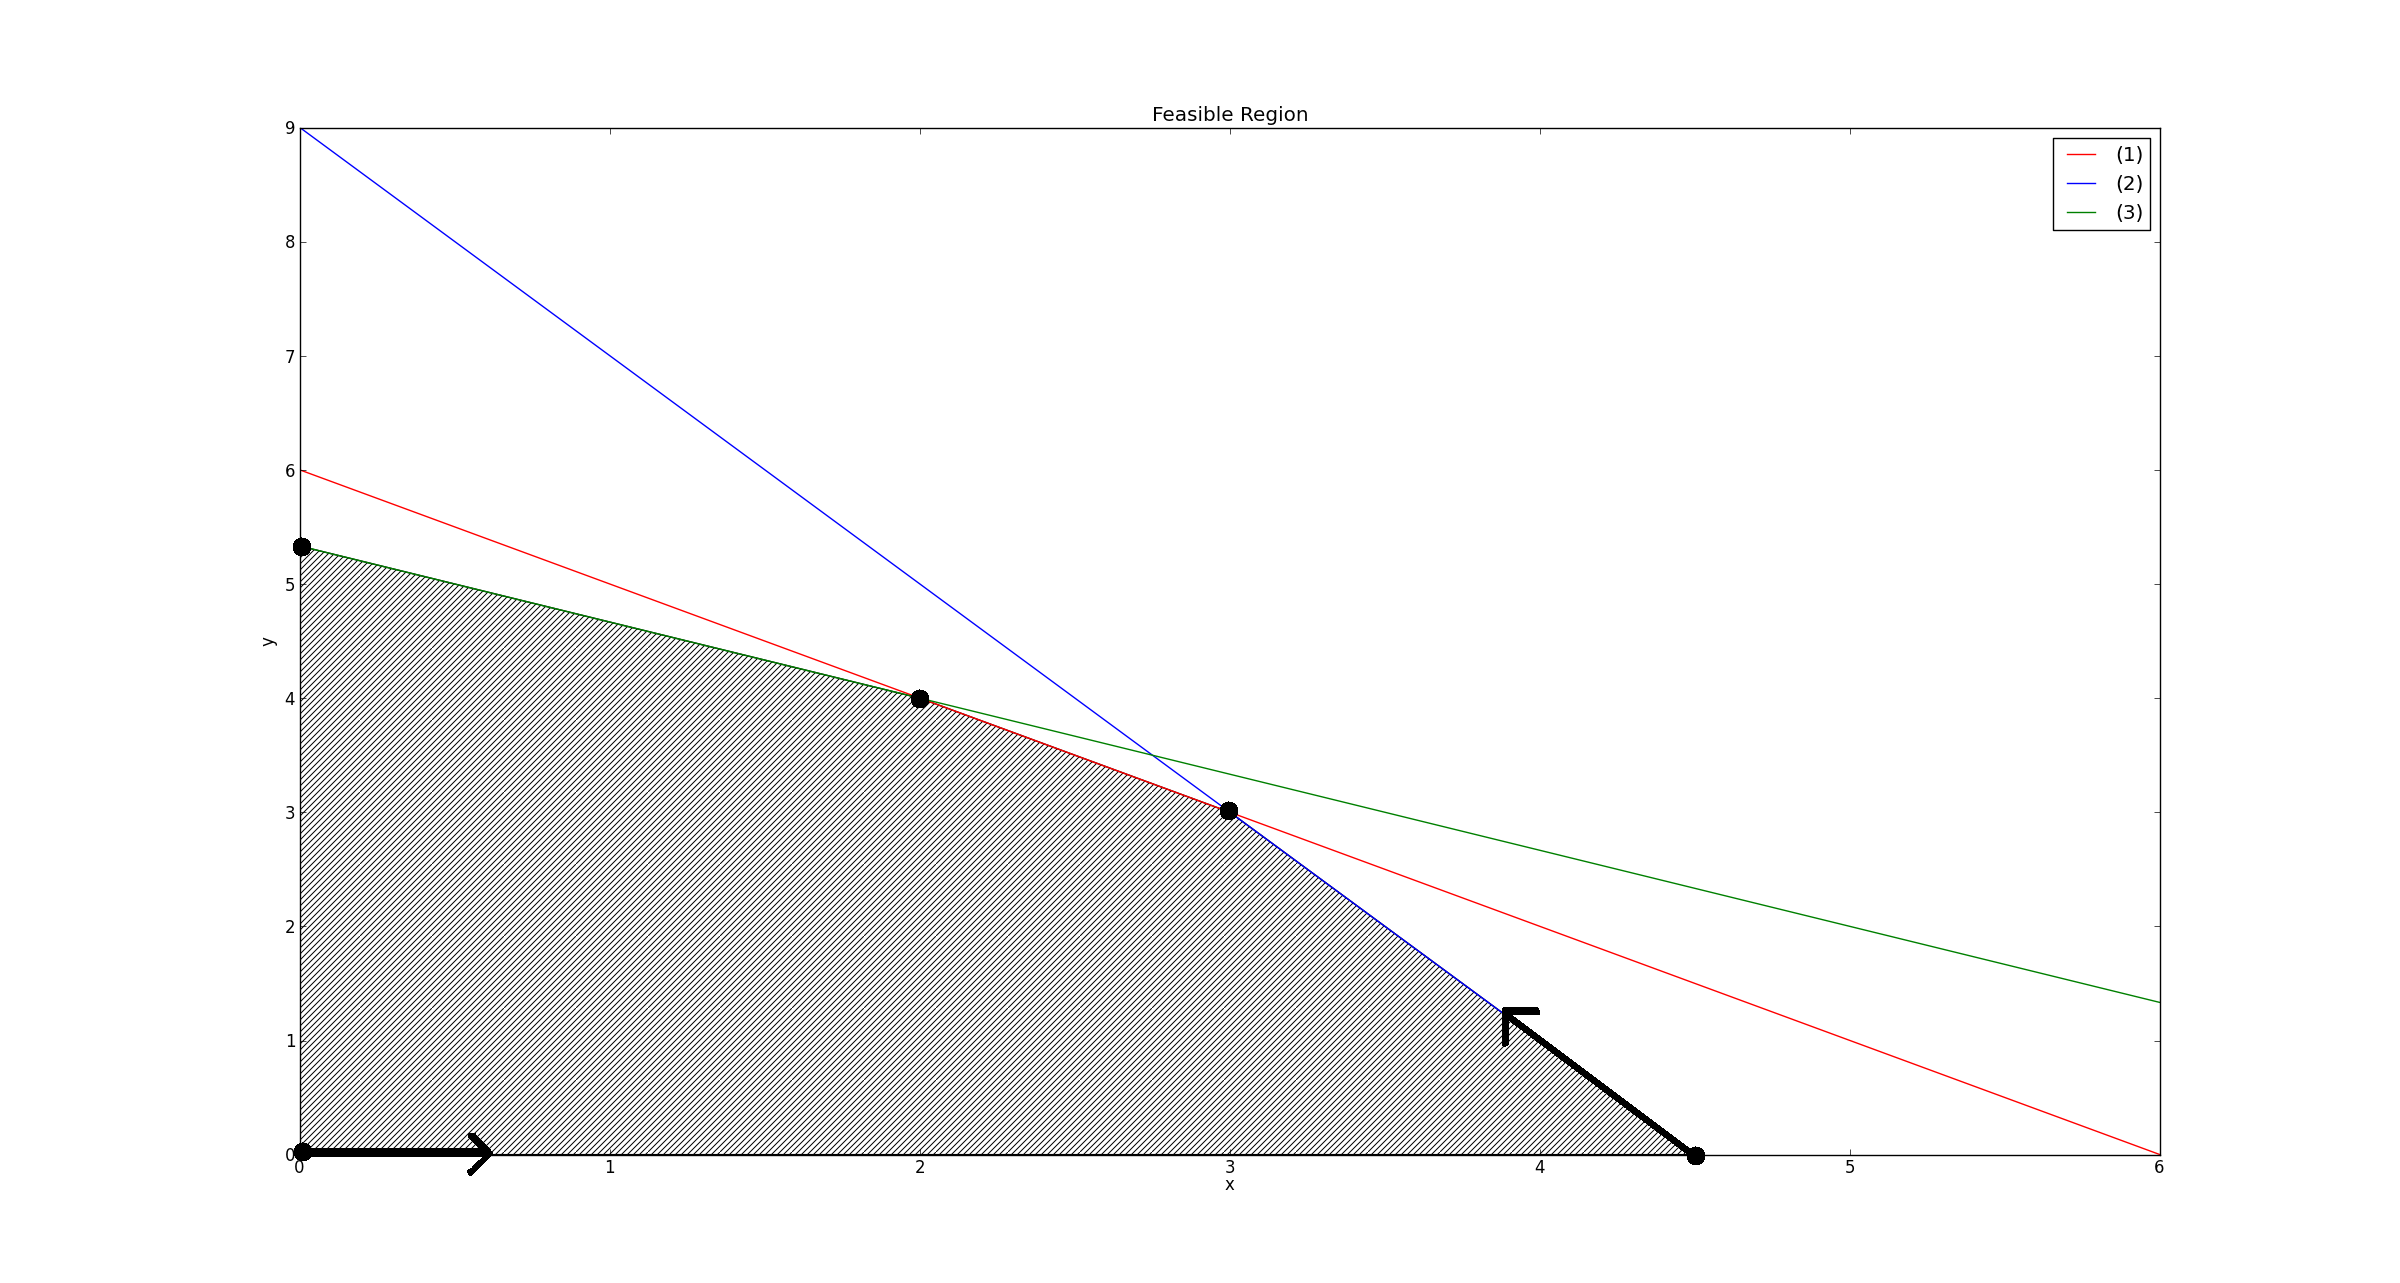
\includegraphics[scale=0.15]{simplex_iterations.png}
\end{frame}

{
\setbeamercolor{background canvas}{bg=exerciseblue}
\begin{frame}
\frametitle{Exercises}
\begin{itemize}
\item Solve the preceding model with Gurobi.
    \begin{itemize}
    \item Note: Set the model attribute ModelSense to -1 in order to maximize
    \end{itemize}
\item Which constraints are tight at the optimal solution?
\item Besides the origin, the feasible region has three other extreme points that are suboptimal under the current objective function. How might you change the objective function coefficients so that:
    \begin{itemize}
    \item the extreme point at $(0, \frac{16}{3})$ is optimal?
    \item the extreme point at $(\frac{9}{2}, 0)$ is optimal?
    \item all points between $(2, 4)$ and $(3, 3)$ are optimal?
    \end{itemize}
\end{itemize}
\end{frame}
}

\begin{frame}
\frametitle{Duality}
The diet problem, revisited:
\begin{itemize}
\item Let's take the perspective of a supplement vendor, who has pills that contain a single unit of iron or calcium that can be used to replace meals.
\item This vendor will attempt sell these pills to a dieter, and must determine the appropriate price to offer.
\item We'll assume the dieter knows how to solve the diet problem and will replace her optimal diet with pills but only if her cost does not increase.
\item How does the vendor determine pill prices that maximize revenue and are competitive with the food types?
\end{itemize}
\end{frame}

\begin{frame}
\frametitle{Duality}
\begin{columns}[t]
\begin{column}{5cm}
\begin{center}
\begin{tabular} {c | c | c | c}
Food & Iron & Calcium & Cost \\
\hline
1 & 2 & 0 & 20 \\
2 & 0 & 1 & 10 \\
3 & 3 & 2 & 31 \\
4 & 1 & 2 & 11 \\
5 & 2 & 1 & 12 \\
\end{tabular}
\end{center}
Nutrient requirements: \\ Iron: 21, Calcium: 12
\end{column}
\begin{column}{6.5cm}
\begin{itemize}
\item Let $\pi_i, \pi_c$ be the price to be charged for an iron, calcium pill.
\item We wish to maximize total revenue of $v = 21 \pi_i + 12 \pi_c$.
\item We must charge prices that are competitive with the prices of the five food types.
    \begin{itemize}
    \item $2\pi_i \le 20$
    \item $\pi_c \le 10$
    \item $3\pi_i + 2\pi_c \le 31$
    \item $\pi_i + 2\pi_c \le 11$
    \item $2\pi_i + \pi_c \le 12$
    \end{itemize}
\end{itemize}
\end{column}
\end{columns}
\end{frame}

\begin{frame}
\frametitle{Duality}
\small
The diet problem:
\begin{eqnarray}
z^* = \min_x && 20x_1 + 10x_2 + 31x_3 + 11x_4 + 12x_5 \nonumber \\
\mbox{s.t.} && 2x_1 + 0x_2 + 3x_3 + 1x_4 + 2x_5 \ge 21 \nonumber \\
&& 0x_1 + 1x_2 + 2x_3 + 2x_4 + 1x_5 \ge 12 \nonumber \\
&& x_j \ge 0,\;\;j=1,2,\ldots, 5 \nonumber
\end{eqnarray}
The ``dual'' problem:
\begin{eqnarray}
v^* = \max_\pi && 21 \pi_i + 12 \pi_c \nonumber \\
\mbox{s.t.} && 2\pi_i + 0\pi_c \le 20 \nonumber \\
&& 0\pi_i + 1\pi_c \le 10 \nonumber \\
&& 3\pi_i + 2\pi_c \le 31 \nonumber \\
&& 1\pi_i + 2\pi_c \le 11 \nonumber \\
&& 2\pi_i + 1\pi_c \le 12 \nonumber \\
&& \pi_i, \pi_c \ge 0 \nonumber
\end{eqnarray}
\end{frame}

{
\setbeamercolor{background canvas}{bg=exerciseblue}
\begin{frame}
\frametitle{Exercises}
\begin{itemize}
\item Intuitively, is it possible for $v^* > z^*$?
\item Solve the dual of the diet problem with Gurobi. (Maintain a copy of the Model object for the original diet problem for comparison purposes.)
\item How are $z^*$ and $v^*$ related?
\item How are $\pi_i^*$ and $\pi_c^*$ related to solution of the original diet problem?
\item Multiply the iron constraint in the original diet problem by $\pi_i^*$, the calcium constraint by $\pi_c^*$, and add the results.
    \begin{itemize}
    \item What is the resulting inequality?
    \item How can this inequality be used to prove optimality?
    \end{itemize}
\end{itemize}
\end{frame}
}

\begin{frame}
\frametitle{Computing Shadow Prices}
Gurobi computes $\pi$ for us even when we solve the primal. Recall that in the optimal solution to the diet problem example, only $x_4$ and $x_5$ were non-zero. Letting $b_i$ and $b_c$ be nutrient requirements, we have
\begin{eqnarray}
x_4 + 2 x_5 &=& b_i \nonumber \\
2 x_4 + x_5 &=& b_c \nonumber
\end{eqnarray}
We can solve for $x_4$ and $x_5$ as
\begin{eqnarray}
x_4 &=& -1/3 b_i + 2/3 b_c \nonumber \\
x_5 &=& 2/3 b_i - 1/3 b_c \nonumber
\end{eqnarray}
Plugging into the objective, we get
\begin{eqnarray}
z &=& 11x_4 + 12 x_5 \nonumber \\
&=& 11(-1/3 b_i + 2/3 b_c) + 12(2/3 b_i - 1/3 b_c) \nonumber \\
&=& 13/3 b_i + 10/3 b_c \nonumber
\end{eqnarray}
So, $\pi_i = 13/3$ and $\pi_c = 10/3$.
\end{frame}

\begin{frame}
\frametitle{Computing Reduced Costs}
\begin{itemize}
\item How are the reduced costs related to the shadow prices?
\item Consider food 3, which costs 31 per ounce and provides 3 units of iron and 2 units of calcium.
\item Iron is priced at 13/3 per unit, calcium at 10/3 per unit.
\item If we discount the cost of food 3 by the value of the nutrients that it provides, we get $31 - 3*(13/3) - 2*(10/3) = 34/3$, which is exactly the reduced cost.
\item What is the reduced cost for food 4?
\item How cheap would food type 3 need to be in order for it to be in our diet?
\item Suppose we introduce a new food that costs 20 per ounce and provides 2 units of iron and 3 units of calcium. Should we include this new food in our diet? Do we need to reoptimize?
\end{itemize}
\end{frame}

\end{document}
